\documentclass[12pt,a4paper]{article}
\usepackage[margin=1.7cm]{geometry}
\usepackage[T1]{fontenc}
\usepackage{lmodern}
\usepackage{microtype}
\usepackage{amsmath}
\usepackage{booktabs,tabularx,array}
\usepackage{tikz}
\usetikzlibrary{arrows.meta,positioning}
\definecolor{navy}{HTML}{1F4E79}
\definecolor{orange}{HTML}{C55A11}
\definecolor{green}{HTML}{548235}
\definecolor{red}{HTML}{B00020}
\pagestyle{empty}
\setlength{\parindent}{0pt}
\begin{document}

{\centering\Large\bfseries Q1 onboarding decision flow\par}
\vspace{1mm}
{\centering\small One-page suitability rule for Profiles A--E.\par}
\vspace{3mm}

\begin{center}
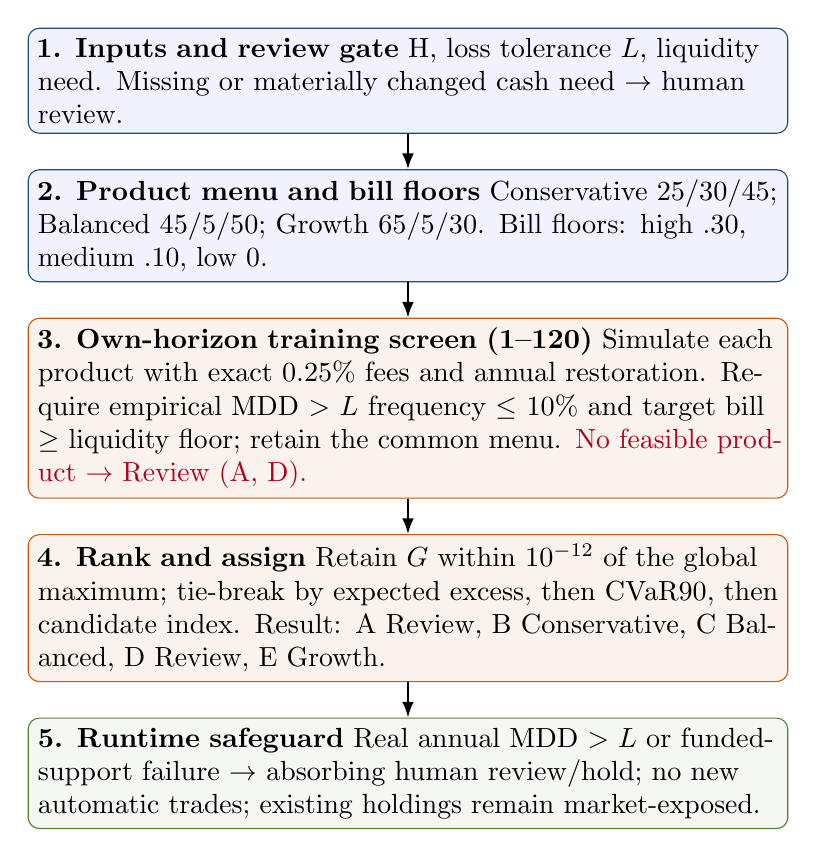
\begin{tikzpicture}[
  node distance=4.5mm,
  box/.style={draw=navy,rounded corners,fill=blue!5,align=left,text width=9.4cm,inner sep=3.5pt},
  decision/.style={draw=orange,rounded corners,fill=orange!8,align=left,text width=9.4cm,inner sep=3.5pt},
  runtime/.style={draw=green,rounded corners,fill=green!6,align=left,text width=9.4cm,inner sep=3.5pt},
  arrow/.style={-{Latex[length=2mm]},thick}
]
\node[box] (input) {\textbf{1. Inputs and review gate}\ H, loss tolerance $L$, liquidity need. Missing or materially changed cash need $\to$ human review.};
\node[box,below=of input] (menu) {\textbf{2. Product menu and bill floors}\ Conservative 25/30/45; Balanced 45/5/50; Growth 65/5/30. Bill floors: high .30, medium .10, low 0.};
\node[decision,below=of menu] (screen) {\textbf{3. Own-horizon training screen (1--120)}\ Simulate each product with exact 0.25\% fees and annual restoration. Require empirical $\mathrm{MDD}>L$ frequency $\le 10\%$ and target bill $\ge$ liquidity floor; retain the common menu. \textcolor{red}{No feasible product $\to$ Review (A, D).}};
\node[decision,below=of screen] (rank) {\textbf{4. Rank and assign}\ Retain $G$ within $10^{-12}$ of the global maximum; tie-break by expected excess, then CVaR90, then candidate index. Result: A Review, B Conservative, C Balanced, D Review, E Growth.};
\node[runtime,below=of rank] (runtime) {\textbf{5. Runtime safeguard}\ Real annual MDD $>L$ or funded-support failure $\to$ absorbing human review/hold; no new automatic trades; existing holdings remain market-exposed.};
\draw[arrow] (input) -- (menu);
\draw[arrow] (menu) -- (screen);
\draw[arrow] (screen) -- (rank);
\draw[arrow] (rank) -- (runtime);
\end{tikzpicture}
\end{center}

\vspace{2mm}
\begin{minipage}[t]{0.48\textwidth}
{\bfseries Development decision trace\par}
\vspace{1mm}
{\small\setlength{\tabcolsep}{2pt}
\begin{tabular}{@{}lcccc@{}}
\toprule
Profile & Risk-feasible & Joint & Menu & Assignment\\
\midrule
A & 0 & 0 & 0 & \textbf{Review}\\
B & 52 & 52 & 1 & \textbf{Conservative}\\
C & 93 & 93 & 2 & \textbf{Balanced}\\
D & 0 & 0 & 0 & \textbf{Review}\\
E & 157 & 92 & 3 & \textbf{Growth}\\
\bottomrule
\end{tabular}}
\end{minipage}\hfill
\begin{minipage}[t]{0.47\textwidth}
{\bfseries What the numbers mean\par}
\vspace{1mm}
{\small
A and D have no risk-feasible product; the liquidity floor alone is not enough.
B/C/E have a common-menu candidate. The 10\% screen is a declared service
reference, not a contest mandate or a guarantee. On final 121--180, B/C static
frequencies rise above 10\% and E Growth has negative P10 growth; these adverse
findings are disclosed, not repaired by changing assignments. Q1 static products
are not the Q2 guarded service.\par}
\end{minipage}

\vfill
{\footnotesize\raggedright\color{black!65}Source: frozen V2b registry; full-development 1--120 feasibility counts. Exact tie-break and hashes: \texttt{service\_refinement\_readiness\_review.json}, \texttt{joint\_liquidity\_refit\_protocol.json}.\par}
\end{document}
